\subsection{Creating particles}

We need to create the particles representing the volume of the water before we run the simulation. To do this we need a function that tells us if a point in space $\vec{x}$ is inside our outside of the initial shape of the water.  We create $c_p$ particles for a two dimensional cell that is completely inside of the water. The initial FLIP report suggests the use of $c_p = 4$ with particles jittered evenly inside the cell. Less particles tend to create gaps in the simulation and more particles create unnecessary noise. 

\begin{algorithm}
\caption{Creating particles from an initial water shape}
\begin{algorithmic}
\FOR{$i=0$ to $N_x$}
\FOR{$j=0$ to $N_y$}
\FOR{$k=0$ to $c_p$}
\STATE p = (i,j)$\cdot \Delta x +\frac{random(-1,1) \cdot \Delta x}{2}$
\IF{p is inside water and $\phi_s(p) > 0$}
\STATE create particle at p
\ENDIF
\ENDFOR
\ENDFOR
\ENDFOR
\end{algorithmic}
\label{createalgorithm}
\end{algorithm}
\noindent
In Algorithm \ref{createalgorithm}, p is a two dimensional vector. {\it random(a,b)} is a function that returns a random value evenly distributed between $a$ and $b$. The $\phi_s > 0$ is a solid level set check to see if the position is outside of the solid. Figure \ref{createexample} shows a basic example of an initial solid level set $\phi_s$ colored grey and an closed water volume in blue.

\begin{figure}[ht!]
\centering
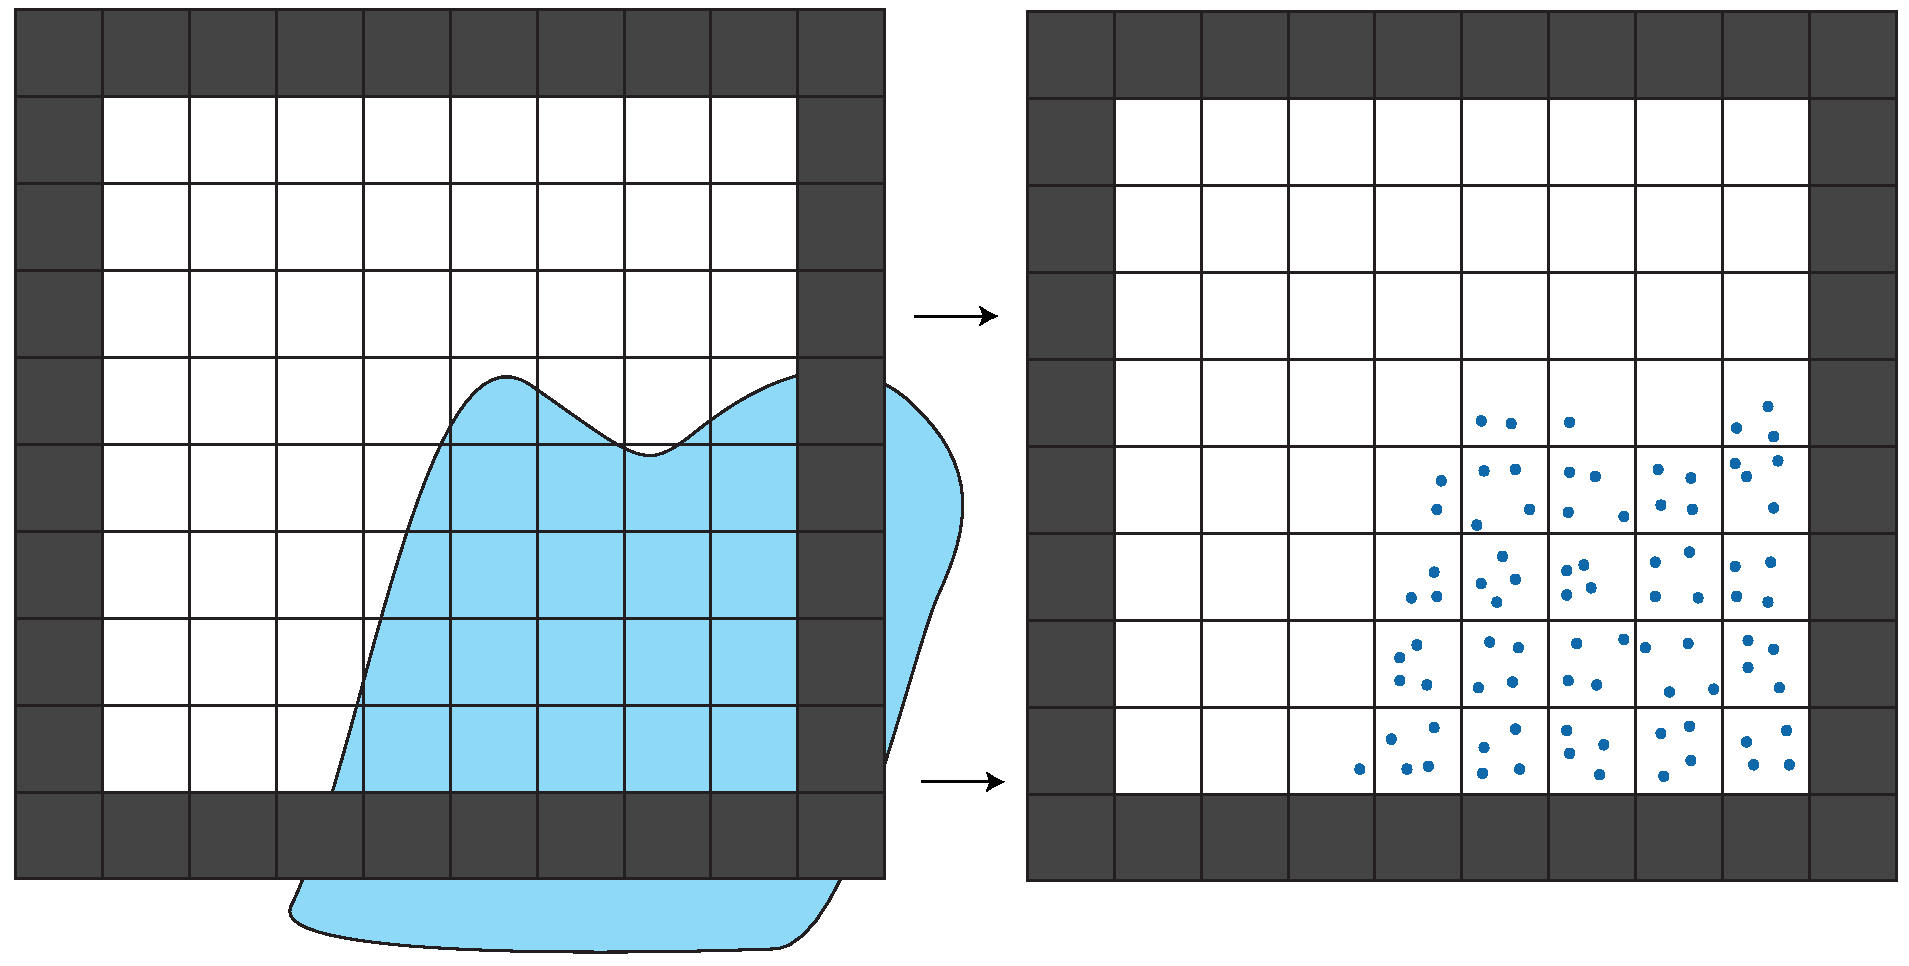
\includegraphics[width=80mm]{img/create.pdf}
\caption{Creating the FLIP particles from a given shape.}
\label{createexample}
\end{figure}


